% Results as coauthor bullet notes, replaced by prose on 2026-10-15 (kept for reference, not compiled)
\section*{Results}

\textbf{Figure 1: Sites and EFP distributions}
\begin{itemize}
  \item \textbf{101 sites, 361 site-years}, 2020--2025, tree cover $\geq$ 30\,\%:
        ENF 49, DBF 30, MF 7, WET 6, EBF 3, CSH 3, OSH 2, WSA 1. Median 4 years per site; 17 sites have a single year.
  \item Quality control: CN-Sb1 and CN-Sb2 (two Saihanba plantations with extreme WUE) and one negative-WUE
        site-year are excluded.
\end{itemize}
\begin{center}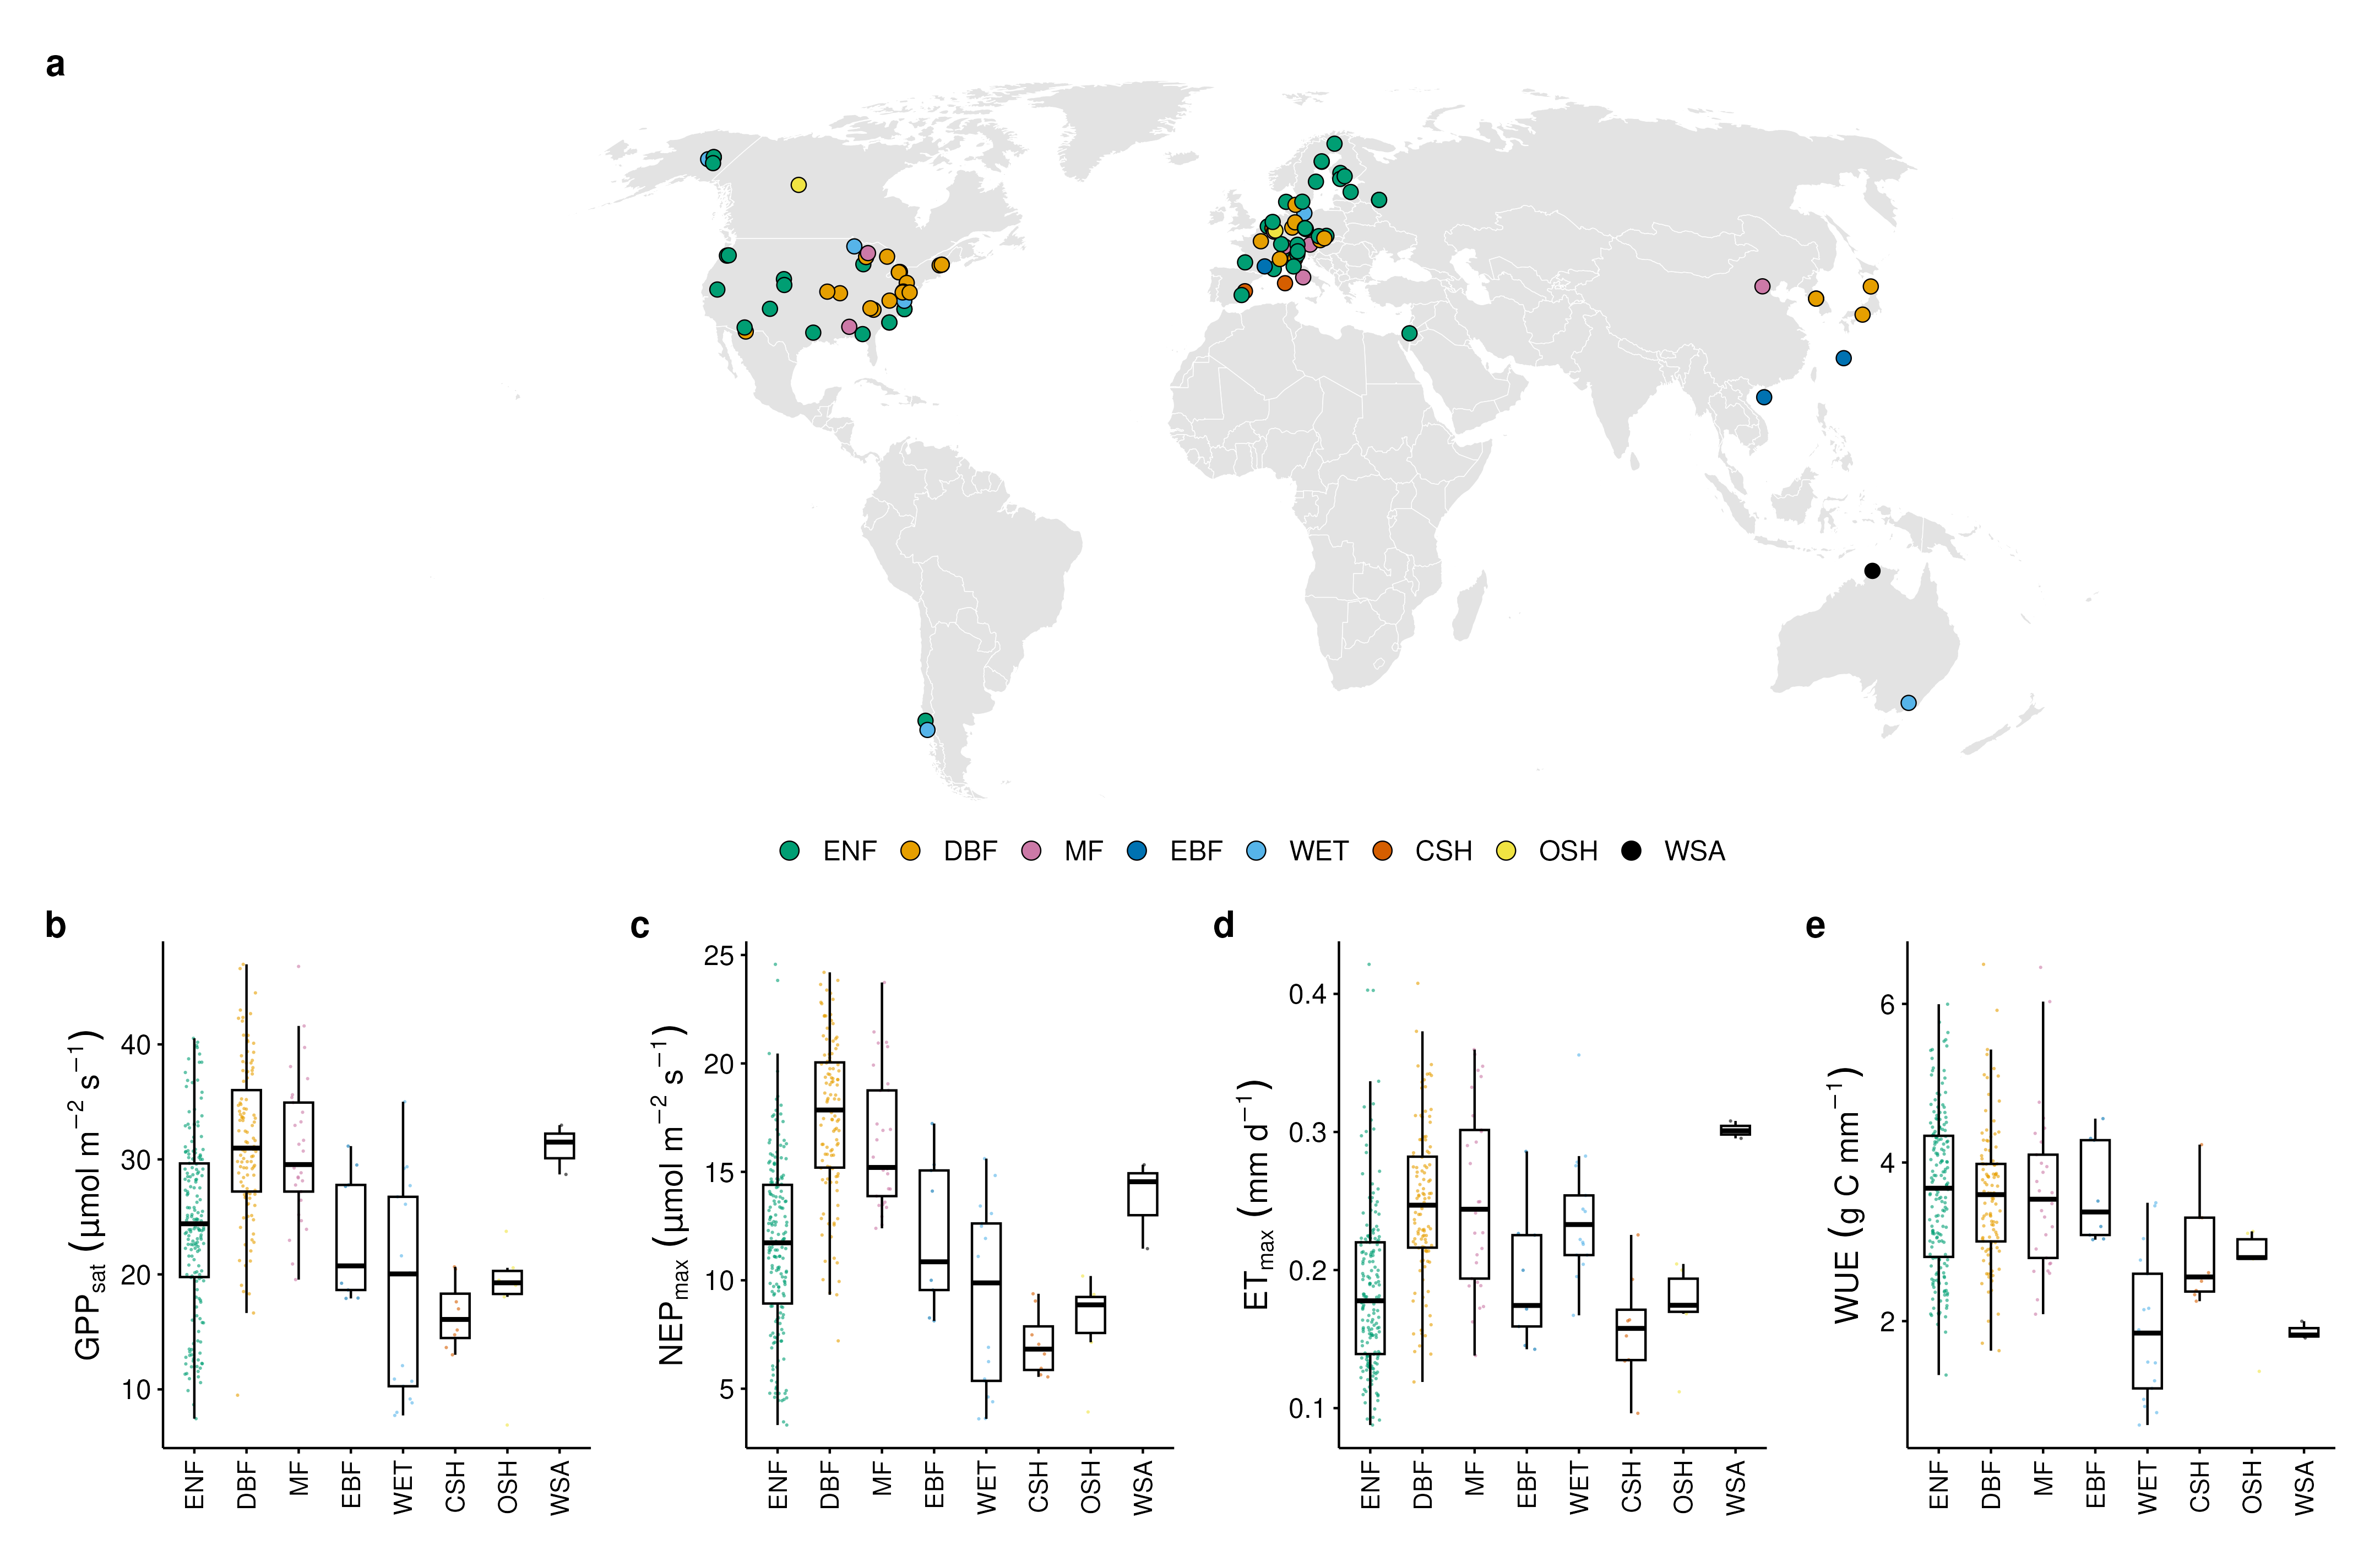
\includegraphics[width=\linewidth]{figures/fig1_site_map.png}\\[2pt]
\parbox{\linewidth}{{\small \textbf{Fig.\ 1} $|$ \textbf{The 101 eddy-covariance sites and their ecosystem functional properties.} \textbf{a}, Sites with at least 30\,\% tree cover, coloured by IGBP vegetation class (ENF, evergreen needleleaf forest; DBF, deciduous broadleaf forest; MF, mixed forest; EBF, evergreen broadleaf forest; WET, wetland; CSH, closed shrubland; OSH, open shrubland; WSA, woody savanna); Robinson projection. \textbf{b--e}, GPP$_\mathrm{sat}$ (\textbf{b}), NEP$_\mathrm{max}$ (\textbf{c}), ET$_\mathrm{max}$ (\textbf{d}) and WUE (\textbf{e}) per vegetation class; points are site-years ($n$ = 361), boxes show the median and interquartile range, whiskers extend to 1.5 times the interquartile range.}}\end{center}

\textbf{Model skill (AutoGluon)}
\begin{itemize}
  \item Repeated leave-one-site-out CV, $R^2$ of climate + traits (C+T) and climate + traits + mortality (C+T+M):
        adding mortality raises the mean $R^2$ from \textbf{0.349 to 0.402} (12\,months) and from \textbf{0.351 to 0.408}
        (24\,months) (Table~\ref{tab:r2}).
  \item Largest gain for NEP$_{max}$ (+0.11), then WUE (+0.06) and GPP$_{sat}$ (+0.04--0.05); ET$_{max}$ unchanged.
  \item AutoGluon is slightly better than XGBoost and LightGBM on average (best in 7 of 16 tasks; Table~\ref{tab:a_r2}).
\end{itemize}

\begin{table}[htbp]
\centering
\caption{\textbf{Adding mortality improves the model skill for three of the four properties.} Coefficient of determination ($R^2$) of repeated leave-one-site-out predictions with climate and traits (C+T) and with mortality added (C+T+M); AutoGluon; $\Delta$, change in $R^2$; 12- and 24-month predictor windows. ET$_\mathrm{max}$ does not improve.}
\label{tab:r2}
\footnotesize
\begin{tabular}{lcccccc}
\toprule
 & \multicolumn{3}{c}{12 months} & \multicolumn{3}{c}{24 months} \\
\cmidrule(lr){2-4}\cmidrule(lr){5-7}
EFP & C+T & C+T+M & $\Delta$ & C+T & C+T+M & $\Delta$ \\
\midrule
GPP$_\mathrm{sat}$ & 0.330 & 0.367 & +0.037 & 0.317 & 0.370 & +0.053 \\
NEP$_\mathrm{max}$ & 0.391 & 0.503 & +0.112 & 0.394 & 0.502 & +0.108 \\
ET$_\mathrm{max}$  & 0.423 & 0.425 & +0.002 & 0.429 & 0.433 & +0.004 \\
WUE                & 0.252 & 0.312 & +0.060 & 0.264 & 0.326 & +0.062 \\
\midrule
Mean               & 0.349 & 0.402 & +0.053 & 0.351 & 0.408 & +0.057 \\
\bottomrule
\end{tabular}
\end{table}

\textbf{Table~\ref{tab:main}: Does mortality reduce the prediction error?} (MAE, site-year level, paired bootstrap)
\begin{itemize}
  \item Every site-year is an observation, so years without mortality do not dilute the years with mortality. Years of
        one site are not independent, so whole sites are resampled (bootstrap) and swapped (paired permutation).
  \item \textbf{Columns.} \emph{All years of the sites}: all 101 sites, the 60 Mid + High sites and the 22 High sites, each
        with all their years (site groups by the site's maximum relative mortality). \emph{Only the years with mortality}:
        site-years whose own relative mortality exceeds 10.6\,\% (Mid + High years) or 24.0\,\% (High years).
  \item \textbf{Mid + High sites, all years} (new column): NEP$_{max}$ $-11.3$ / $-10.5$\,\%, GPP$_{sat}$ $-6.1$ / $-8.3$\,\%,
        WUE $-6.8$ / $-6.4$\,\% (12 / 24\,months; all significant), ET$_{max}$ not significant.
  \item \textbf{NEP$_{max}$: yes, robustly.} MAE $-11.8$ / $-10.8$\,\% over all site-years (12 / 24\,months), $-17.5$ to
        $-22.6$\,\% at High sites and \textbf{$-29$ to $-32$\,\% in high-mortality years}; significant in 7 of 8 cells.
  \item \textbf{WUE: only where mortality happened.} $-4$ to $-5$\,\% over all site-years (n.s.), but $-11$ to $-15$\,\% at
        High sites and $-17$ to $-22$\,\% in high-mortality years, all significant.
  \item \textbf{GPP$_{sat}$: smaller} ($-4$ to $-12$\,\%), significant over all site-years at 24\,months and in the
        Mid + High years; at High sites and in High years the intervals are wide (few site-years).
  \item \textbf{ET$_{max}$: small} ($-1$ to $-11$\,\%), significant only in the Mid + High years at 24\,months.
  \item \textbf{The effect is largest in the years when mortality happened}: for every EFP the error reduction in High
        years is at least twice the one over all site-years (NEP$_{max}$ about 2.7 times).
  \item The bootstrap intervals and the permutation tests agree: every significant cell has its 95\,\% interval entirely
        below zero.
  \item Robustness (Appendix): site-level tests (per-site MAE; log-ratio permutation and site-level bootstrap), RMSE
        instead of MAE, XGBoost and LightGBM, sites weighted by their number of years, one-year sites dropped. NEP$_{max}$
        improves in all of them.
\end{itemize}

\begin{table}[htbp]
\centering
\caption{\textbf{Adding mortality reduces the prediction error (MAE), most in the years in which trees died.} Change in the MAE when the mortality predictors are added to climate and traits (C+T $\rightarrow$ C+T+M), AutoGluon, leave-one-site-out predictions: 100\,(MAE$_\mathrm{C+T+M}$ / MAE$_\mathrm{C+T}$ $-$ 1)\,\%; negative = smaller error. Brackets: 95\,\% interval of a bootstrap that resamples whole sites (10\,000 draws). Stars: one-sided paired permutation test with the two models swapped per site (10\,000 draws), Benjamini--Hochberg corrected across all tests of the same level: $^{*}$\,$q<0.05$, $^{**}$\,$q<0.01$, $^{***}$\,$q<0.001$. \emph{Site-year level}: every site-year is one observation. Columns: all site-years, and only the site-years whose own relative mortality exceeds 10.6\,\% or 24.0\,\% (high mortality). Numbers under the column heads: sites / site-years. 101 sites, 361 site-years, deadtrees v5 maps.}
\label{tab:main}
\scriptsize
\setlength{\tabcolsep}{3pt}
\resizebox{\linewidth}{!}{%
\begin{tabular}{llccc}
\toprule
 & & All site-years & \multicolumn{2}{c}{Only the years with mortality} \\
\cmidrule(lr){4-5}
 & & & $>$ 10.6\,\% & $>$ 24.0\,\% (high mortality) \\
 & & (101 / 361) & (60 / 160) & (22 / 40) \\
\midrule
\multirow{4}{*}{\shortstack[l]{AutoGluon\\12\,months}} & GPP$_\mathrm{sat}$ & $-4.1$ {\tiny[$-8.0$, $-0.2$]}$^{*}$ & $-6.7$ {\tiny[$-12.8$, $-0.7$]}$^{*}$ & $-12.0$ {\tiny[$-29.5$, $+4.9$]} \\
 & NEP$_\mathrm{max}$ & $-11.8$ {\tiny[$-17.0$, $-6.3$]}$^{**}$ & $-12.5$ {\tiny[$-20.1$, $-4.9$]}$^{**}$ & $-31.6$ {\tiny[$-43.2$, $-16.0$]}$^{*}$ \\
 & ET$_\mathrm{max}$ & $-1.3$ {\tiny[$-4.2$, $+1.3$]} & $-3.9$ {\tiny[$-7.7$, $+0.0$]}$^{*}$ & $-9.7$ {\tiny[$-20.6$, $+2.7$]} \\
 & WUE & $-4.3$ {\tiny[$-8.1$, $-0.2$]}$^{*}$ & $-7.2$ {\tiny[$-12.2$, $-1.8$]}$^{*}$ & $-16.9$ {\tiny[$-25.2$, $-5.1$]}$^{*}$ \\
\midrule
\multirow{4}{*}{\shortstack[l]{AutoGluon\\24\,months}} & GPP$_\mathrm{sat}$ & $-5.7$ {\tiny[$-9.5$, $-1.7$]}$^{*}$ & $-8.3$ {\tiny[$-14.2$, $-2.6$]}$^{*}$ & $-11.1$ {\tiny[$-28.0$, $+8.1$]} \\
 & NEP$_\mathrm{max}$ & $-10.8$ {\tiny[$-16.0$, $-5.1$]}$^{**}$ & $-11.6$ {\tiny[$-19.8$, $-2.7$]}$^{*}$ & $-29.2$ {\tiny[$-42.9$, $-8.6$]}$^{*}$ \\
 & ET$_\mathrm{max}$ & $-2.0$ {\tiny[$-5.0$, $+0.9$]} & $-5.4$ {\tiny[$-9.6$, $-1.3$]}$^{*}$ & $-11.4$ {\tiny[$-23.7$, $+3.2$]} \\
 & WUE & $-4.7$ {\tiny[$-9.1$, $-0.1$]}$^{*}$ & $-8.2$ {\tiny[$-14.5$, $-1.5$]}$^{*}$ & $-21.8$ {\tiny[$-34.5$, $-8.2$]}$^{*}$ \\
\bottomrule
\end{tabular}}
\end{table}


\textbf{Figure 2: Without mortality the model predicts too high in high-mortality years}
\begin{itemize}
  \item Every \textbf{site-year} is an observation, grouped by the relative mortality of that year (so the years in which
        mortality happened are not averaged with undisturbed years); y = mean residual (observed $-$ predicted), below 0 = the
        model predicts too high.
  \item \textbf{Without mortality (C+T)} the model over-predicts in the $>$30\,\% class (21 site-years, 10 sites):
        NEP$_{max}$ by $-4.0$\,$\mu$mol\,m$^{-2}$\,s$^{-1}$ [$-5.5$, $-2.4$], GPP$_{sat}$ by $-4.3$ [$-7.5$, $-1.3$],
        WUE by $-0.77$\,g\,C\,mm$^{-1}$ [$-1.10$, $-0.29$] (AutoGluon, 24\,months; 95\,\% site-block bootstrap).
        In the low classes the residual is close to 0.
  \item \textbf{With mortality (C+T+M)} the over-prediction shrinks by about two-thirds (NEP$_{max}$ $-1.3$, GPP$_{sat}$
        $-1.1$, WUE $-0.43$) and the intervals include 0. ET$_{max}$ shows no pattern.
  \item \textbf{The correction is significant.} Per site-year, correction = residual with $-$ residual without mortality
        (= how much adding mortality lowers the prediction). In the $>$30\,\% class: GPP$_{sat}$ +3.2, NEP$_{max}$ +2.7,
        WUE +0.34 (all $q<0.01$, paired permutation with sites swapped as blocks); in the 0--10\,\% class mortality
        slightly \emph{raises} the predictions ($-0.8$, $-0.7$, $-0.10$). The correction grows with relative mortality
        (mixed model, per +10\,\%: GPP$_{sat}$ +0.96, NEP$_{max}$ +0.75, WUE +0.10; all $q<0.001$, site-block bootstrap).
        XGBoost and LightGBM: the same, all significant, with smaller corrections (about half; Appendix~A7).
  \item \textbf{Mixed model on the residuals} (residual $\sim$ relative mortality of the year, random intercept per site; all
        361 site-years): without mortality the residual falls by $-0.77$ (NEP$_{max}$), $-0.18$ (WUE) and $-0.59$
        (GPP$_{sat}$) per +10\,\% relative mortality; robust to a site-block bootstrap, to leaving out any single site and to
        removing the three sites with $>$50\,\% relative mortality. With mortality the trend is no longer significant (Appendix~A7).
  \item The result comes mostly from the few site-years with $>$30\,\% relative mortality --- the years in which mortality happened.
\end{itemize}

\begin{center}
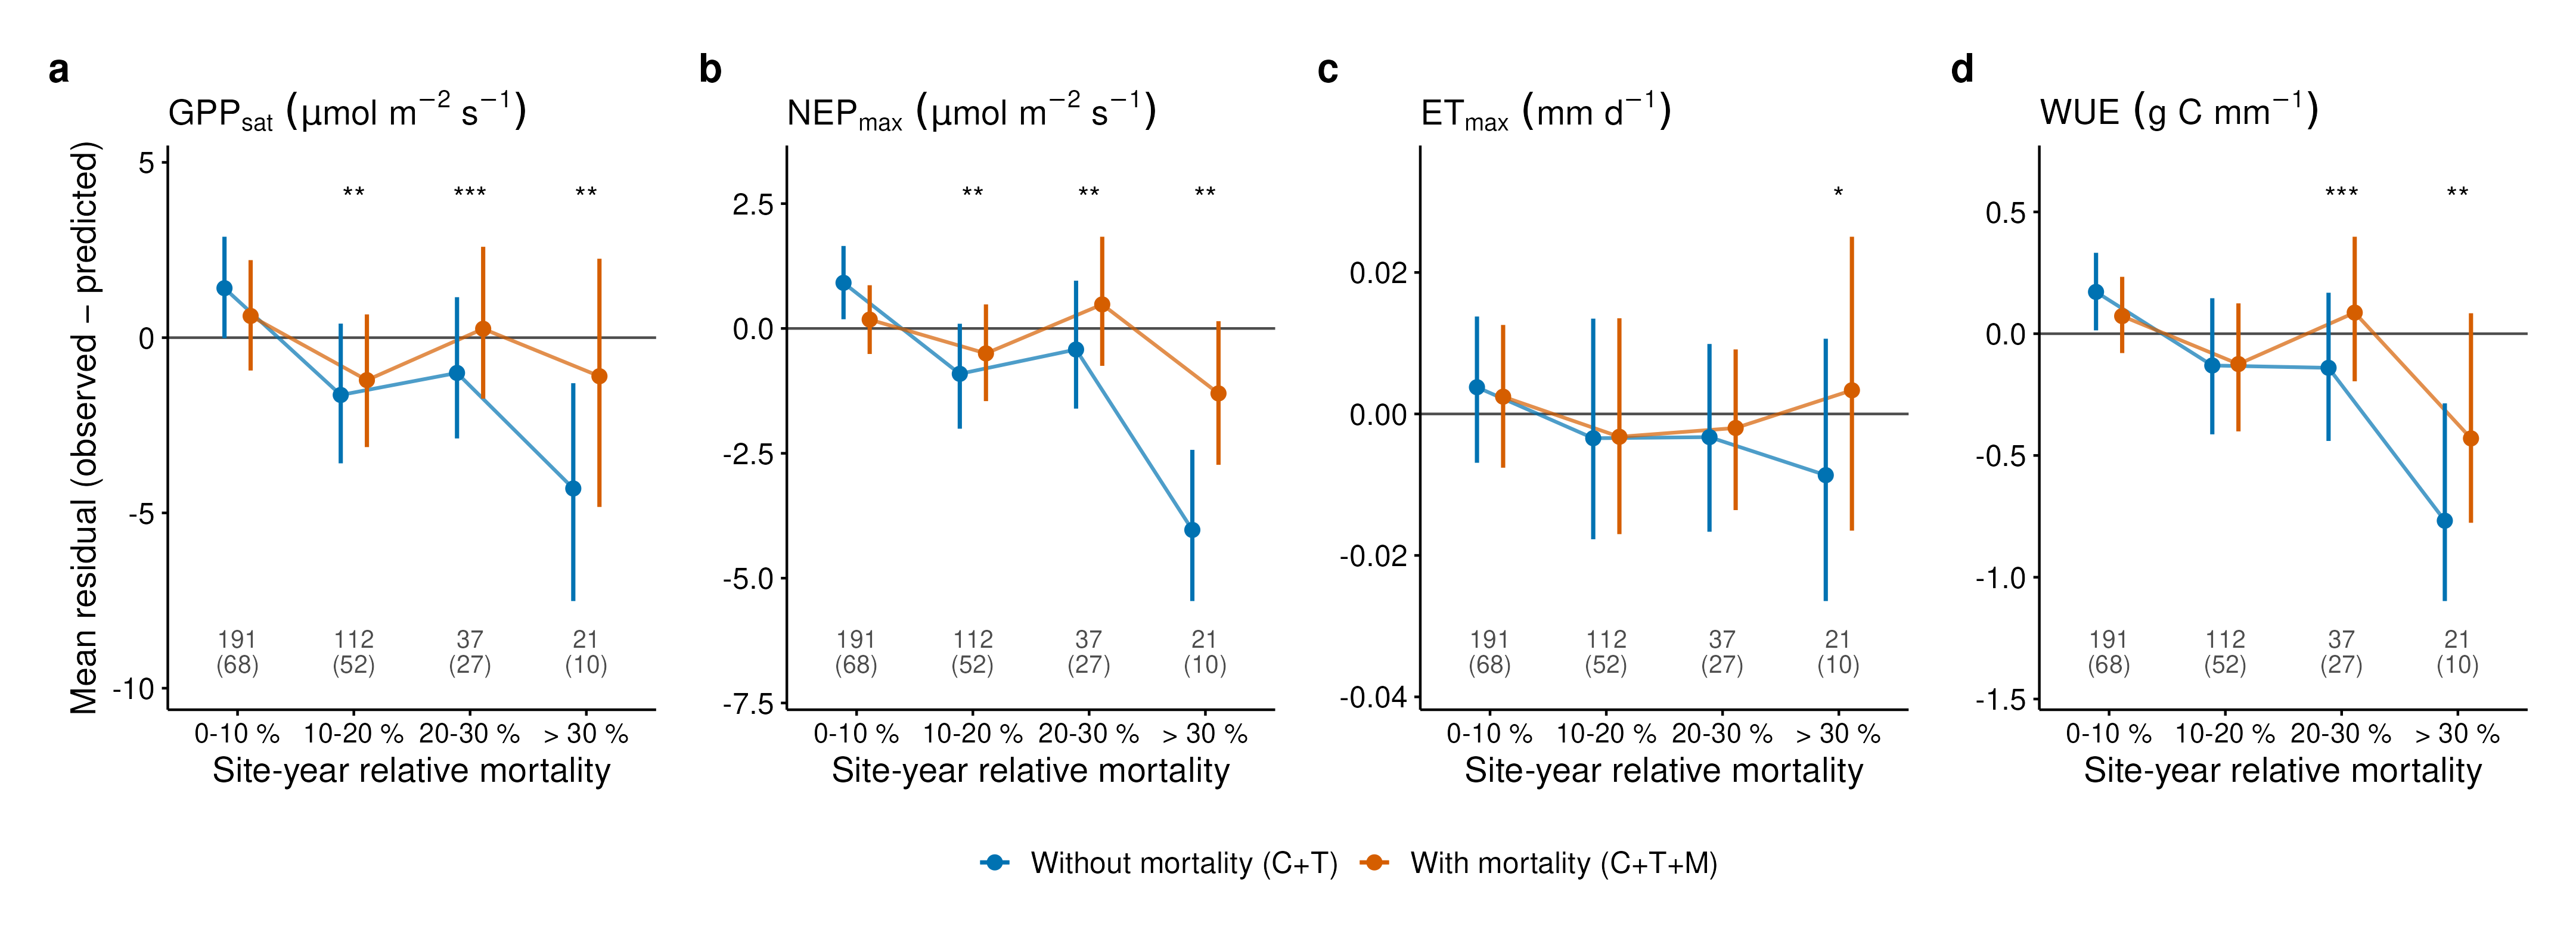
\includegraphics[width=\linewidth]{figures/fig2_residual_by_mortality_AG_24m.png}\\[2pt]
\parbox{\linewidth}{{\small \textbf{Fig.\ 2} $|$ \textbf{Without mortality, the model over-predicts the ecosystem functional properties in years with high mortality.} Mean residual (observed $-$ predicted) of the leave-one-site-out predictions of GPP$_\mathrm{sat}$ (\textbf{a}), NEP$_\mathrm{max}$ (\textbf{b}), ET$_\mathrm{max}$ (\textbf{c}) and WUE (\textbf{d}), grouped by the relative mortality of the site-year, for the model with climate and traits (C+T, blue) and with mortality added (C+T+M, vermillion); AutoGluon, 24-month window. Negative values mean that the model predicts too high. Points, mean; bars, 95\,\% bootstrap interval with whole sites resampled; numbers, site-years (sites) per class. Stars: adding mortality lowers the prediction in that class (one-sided paired permutation test with the two models swapped per site, Benjamini--Hochberg corrected; $^{*}$\,$q<0.05$, $^{**}$\,$q<0.01$, $^{***}$\,$q<0.001$).}}
\end{center}

\textbf{Figure 3: Direction of the mortality effect at each site} (signed SHAP, relative mortality, 24 months)
\begin{itemize}
  \item C+T+M model, per site the \textbf{net signed SHAP of the mortality block} (sum over the mortality predictors,
        averaged over the site's years, response units). Sites sorted by their maximum \textbf{relative mortality} (mean
        of the five buffers), highest on the left; dashed lines = Low / Mid / High breaks (10.6\,\% and 24.0\,\%).
        Below zero = the model predicts a \emph{lower} EFP at that site because of its mortality values.
  \item \textbf{The sign follows the mortality class.} Share of sites with a negative contribution, Low / Mid / High:
        GPP$_{sat}$ 7 / 66 / 86\,\%; NEP$_{max}$ 10 / 68 / 91\,\%; WUE 2 / 58 / 86\,\%; ET$_{max}$ 24 / 50 / 77\,\%.
  \item \textbf{Size:} median $-2.1$ (GPP$_{sat}$) and $-1.5$ (NEP$_{max}$) $\mu$mol\,m$^{-2}$\,s$^{-1}$ at High
        sites, $+1.4$ and $+1.2$ at Low sites; ET$_{max}$ contributions are tiny ($\pm$0.005\,mm\,d$^{-1}$).
  \item Overall importance (share of mean $|$SHAP$|$, C+T+M): mortality 24\,\% (GPP$_{sat}$), 28\,\% (NEP$_{max}$),
        16\,\% (ET$_{max}$), 23\,\% (WUE); climate 52--66\,\%; traits 11--20\,\%.
  \item The version with site names, the 12-month window and XGBoost / LightGBM are in the Appendix.
\end{itemize}

\begin{center}
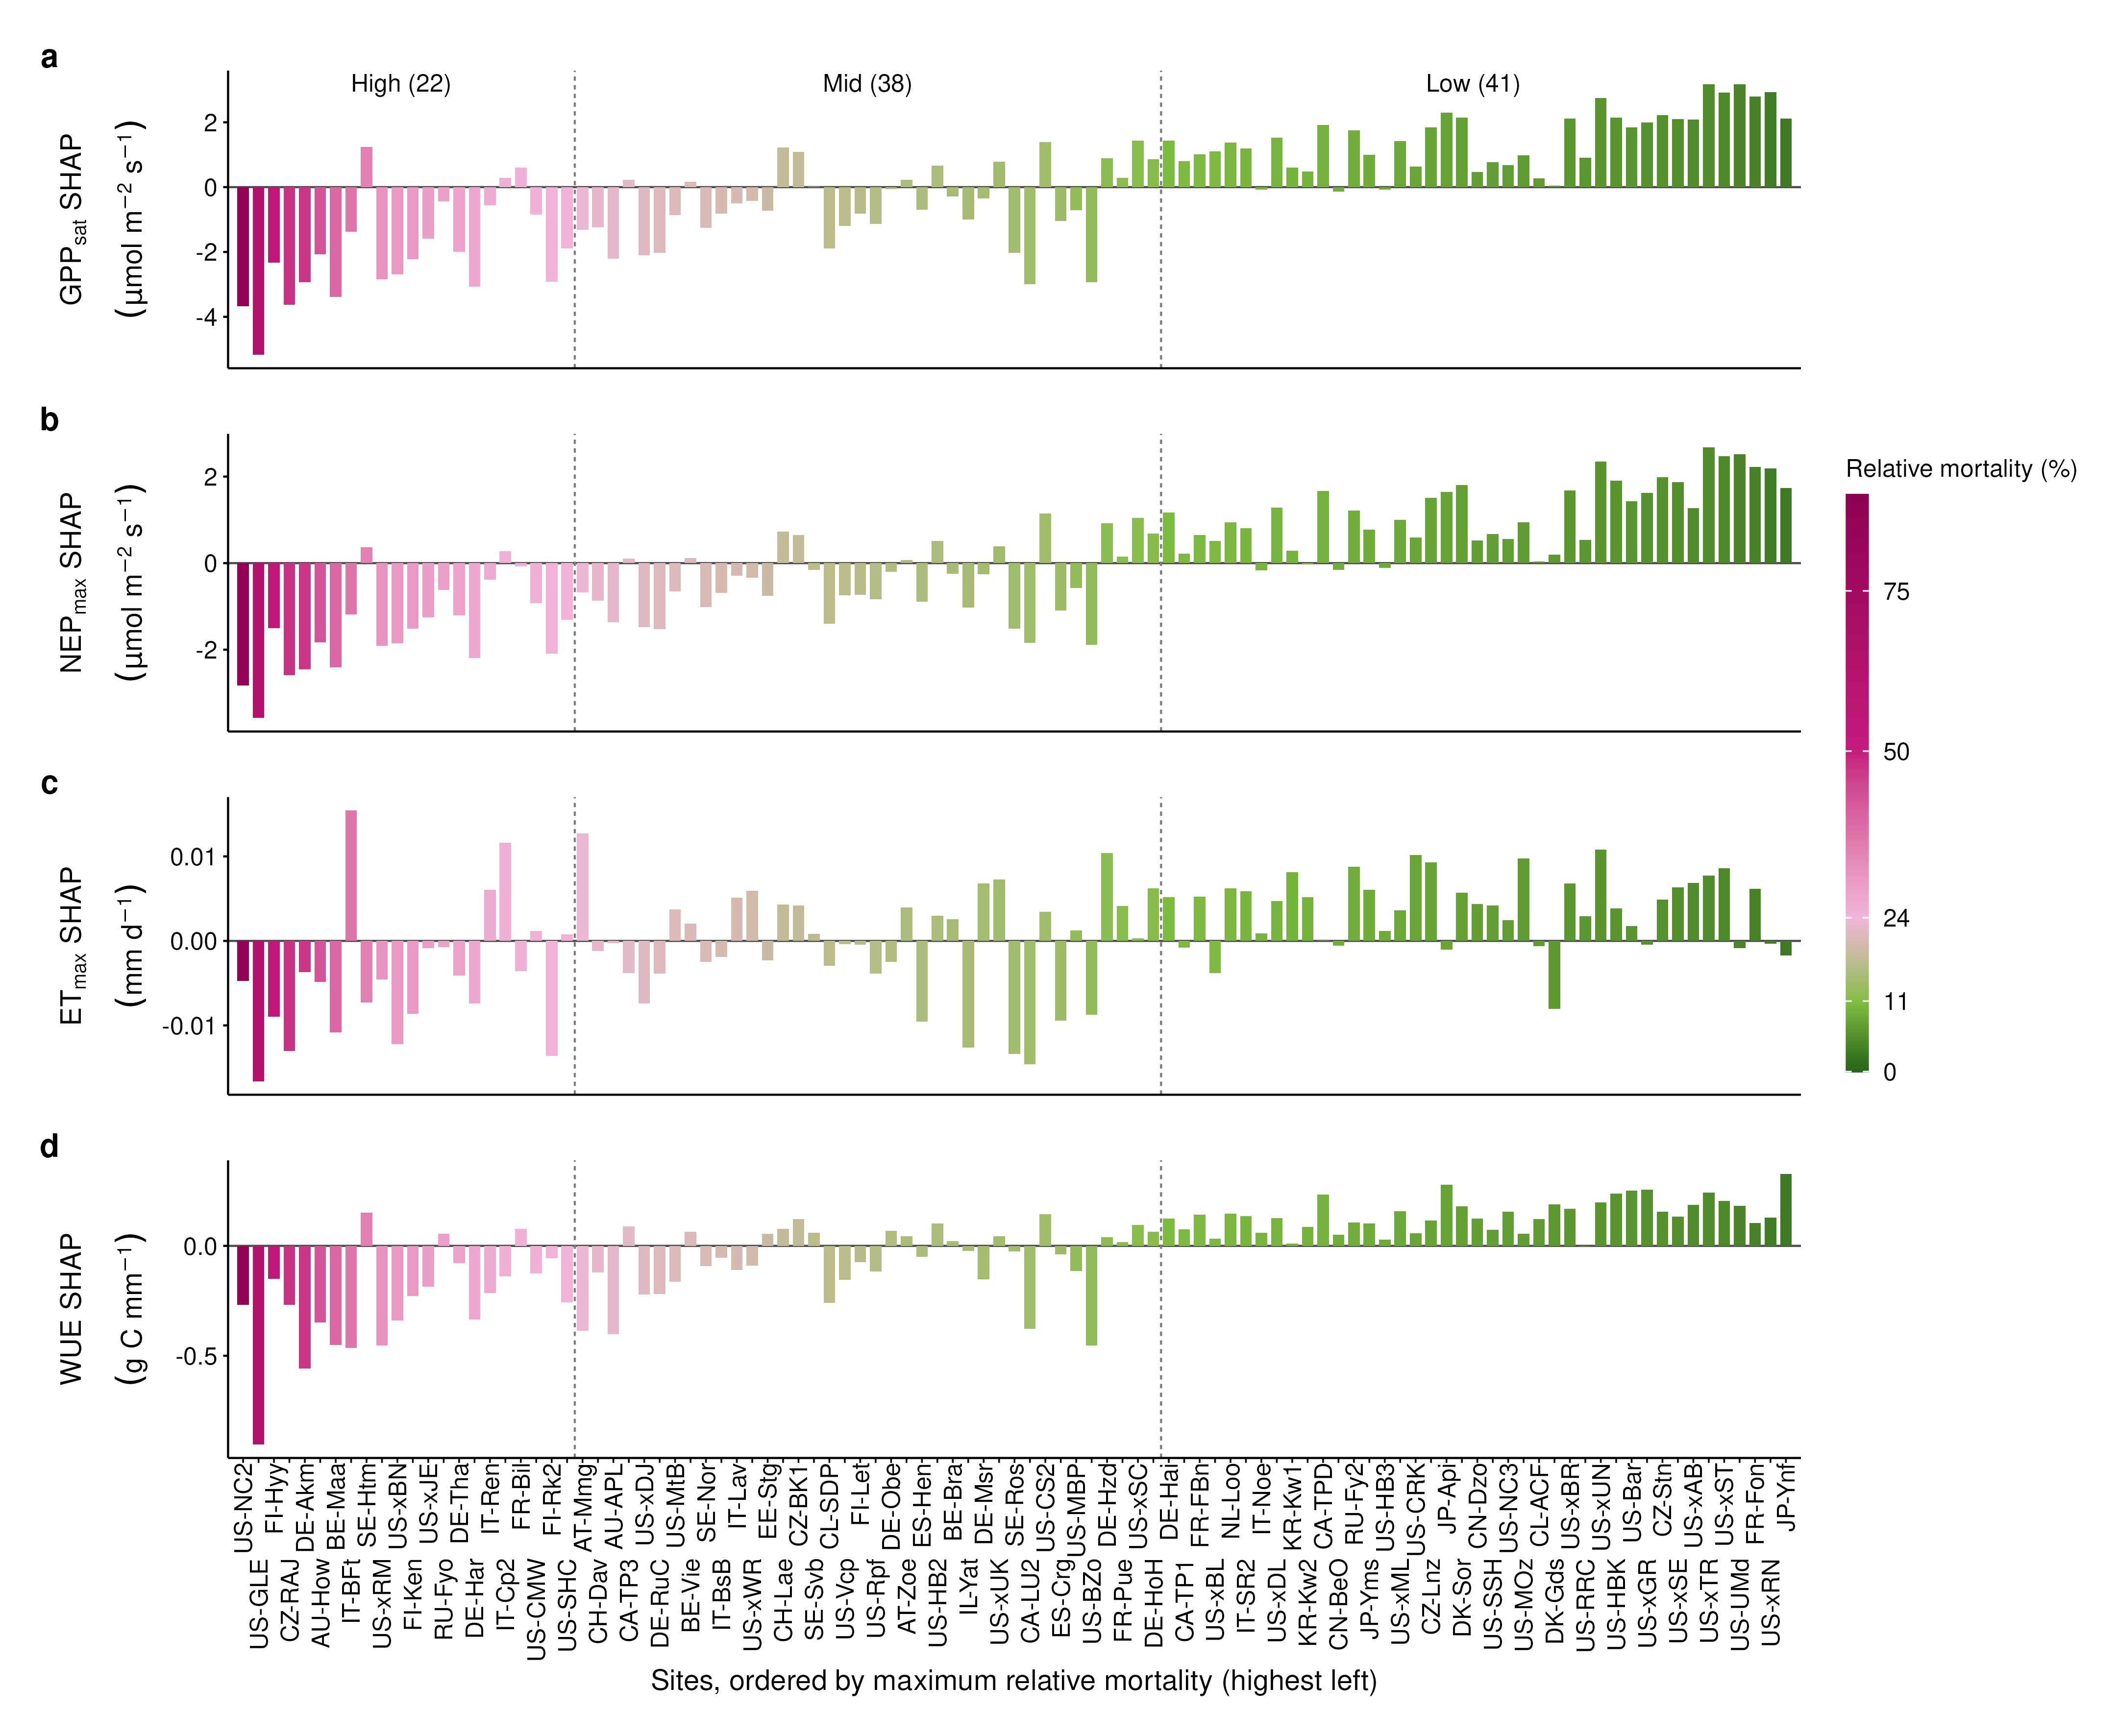
\includegraphics[width=\linewidth]{figures/fig3_signed_relmort_24m_AG_piyg_names.png}\\[2pt]
\parbox{\linewidth}{{\small \textbf{Fig.\ 3} $|$ \textbf{Mortality lowers the predicted carbon uptake and water-use efficiency at sites with high mortality and raises them slightly where mortality is low.} Net contribution of the mortality predictors (sum of their SHAP values, mean over the years of each site) to the predicted GPP$_\mathrm{sat}$ (\textbf{a}), NEP$_\mathrm{max}$ (\textbf{b}), ET$_\mathrm{max}$ (\textbf{c}) and WUE (\textbf{d}), in the units of each property; model with climate, traits and mortality (C+T+M), AutoGluon, 24-month window. Negative values: mortality lowers the prediction at that site. The 101 sites are ordered by their maximum relative mortality (mean of five buffers of 100--500\,m radius), highest on the left, and coloured from green (low) to pink (high), with the colour change anchored at the class breaks (dashed lines, 10.6\,\% and 24.0\,\%; number of sites per class in brackets). FLUXNET site codes below the panels.}}
\end{center}

\textbf{Figure 4: Does the direction differ between High and Low+Mid sites?} (signed SHAP)
\begin{itemize}
  \item \textbf{Below zero means the model predicts a LOWER value of the EFP} (not that it predicts less accurately).
        Classes: site maximum of relative mortality; High $>$ mean + 0.5\,SD (22 High vs 79 Low+Mid). Mann--Whitney U,
        BH-FDR across the figure.
  \item \textbf{A clear dose--response.} At \textbf{High}-mortality sites the block pushes predicted carbon uptake
        \emph{down}; at \textbf{Low+Mid} sites slightly \emph{up} (relative to the average site).
  \item GPP$_{sat}$: High $-1.83$ / $-2.15$, Low+Mid $+0.47$ / $+0.66$ $\mu$mol\,m$^{-2}$\,s$^{-1}$ (12 / 24\,m);
        NEP$_{max}$: High $-1.61$ / $-1.51$, Low+Mid $+0.37$ / $+0.51$; WUE: High $-0.22$ / $-0.24$, Low+Mid
        $+0.07$ g\,C\,mm$^{-1}$; ET$_{max}$: tiny ($-0.003$ / $-0.005$\,mm\,d$^{-1}$). All 8 tests $q<0.001$.
  \item \textbf{Read with Table~\ref{tab:main}:} mortality improves accuracy by lowering predictions at damaged sites.
        Sites are grouped by the same variables whose contribution is measured, so the test confirms that the learned
        relationship is consistent; the direction and size are the informative part.
\end{itemize}

\begin{center}
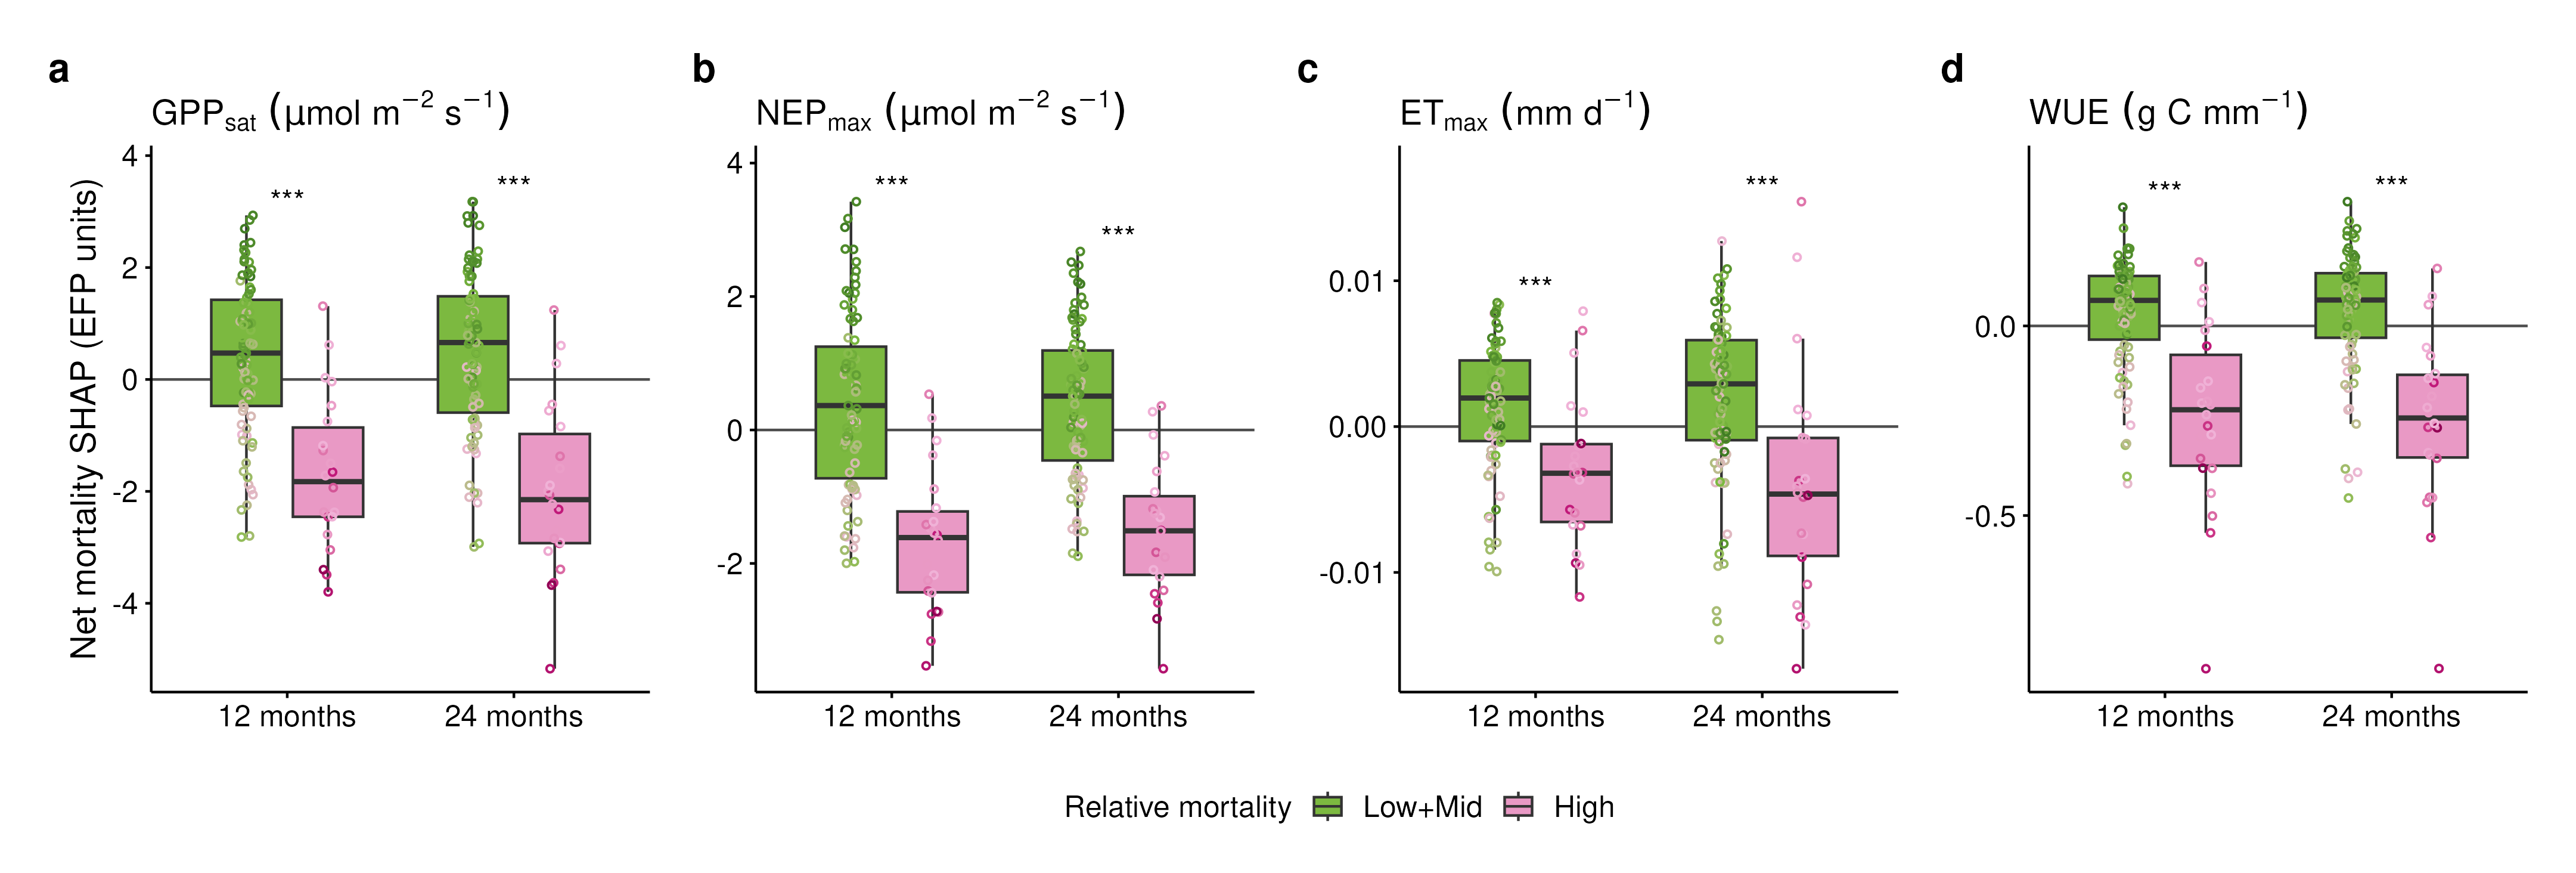
\includegraphics[width=\linewidth]{figures/fig4_relmort_high_vs_lowmid_AG.png}\\[2pt]
\parbox{\linewidth}{{\small \textbf{Fig.\ 4} $|$ \textbf{The direction of the mortality effect differs between high- and low-mortality sites.} Net mortality SHAP per site (as in Fig.~3) at sites with high relative mortality (High, site maximum $>$ 24.0\,\%, $n$ = 22, pink) and at the other sites (Low+Mid, $n$ = 79, green) for GPP$_\mathrm{sat}$ (\textbf{a}), NEP$_\mathrm{max}$ (\textbf{b}), ET$_\mathrm{max}$ (\textbf{c}) and WUE (\textbf{d}), 12- and 24-month windows; AutoGluon, C+T+M. Points are sites in their Fig.~3 colour; box colour, the Fig.~3 colour at the group's median relative mortality; boxes show the median and interquartile range, whiskers extend to 1.5 times the interquartile range. Stars: two-sided Mann--Whitney $U$ test, Benjamini--Hochberg corrected across the eight tests ($^{*}$\,$q<0.05$, $^{**}$\,$q<0.01$, $^{***}$\,$q<0.001$).}}
\end{center}

\textbf{Figure 5: The direction tracks relative mortality}
\begin{itemize}
  \item Per site, net signed mortality SHAP against the site's maximum relative mortality (AutoGluon, C+T+M, 24\,months);
        linear fit with 95\,\% CI, Spearman test.
  \item \textbf{Strong and negative for the carbon fluxes and WUE:} $\rho$ = $-0.81$ (GPP$_{sat}$), $-0.83$ (NEP$_{max}$),
        $-0.78$ (WUE); weaker for ET$_{max}$ ($-0.47$); all $p<0.001$. More mortality, lower predicted carbon uptake.
  \item Sites with little mortality get a positive push, so the sign changes at roughly 10--20\,\% relative mortality.
  \item The benefit itself (error reduction) does not depend on tree cover ($\rho$ = 0.10--0.18, n.s.), and the direction
        tracks mortality more closely than ecosystem type or tree cover (full board in the Appendix).
\end{itemize}

\begin{center}
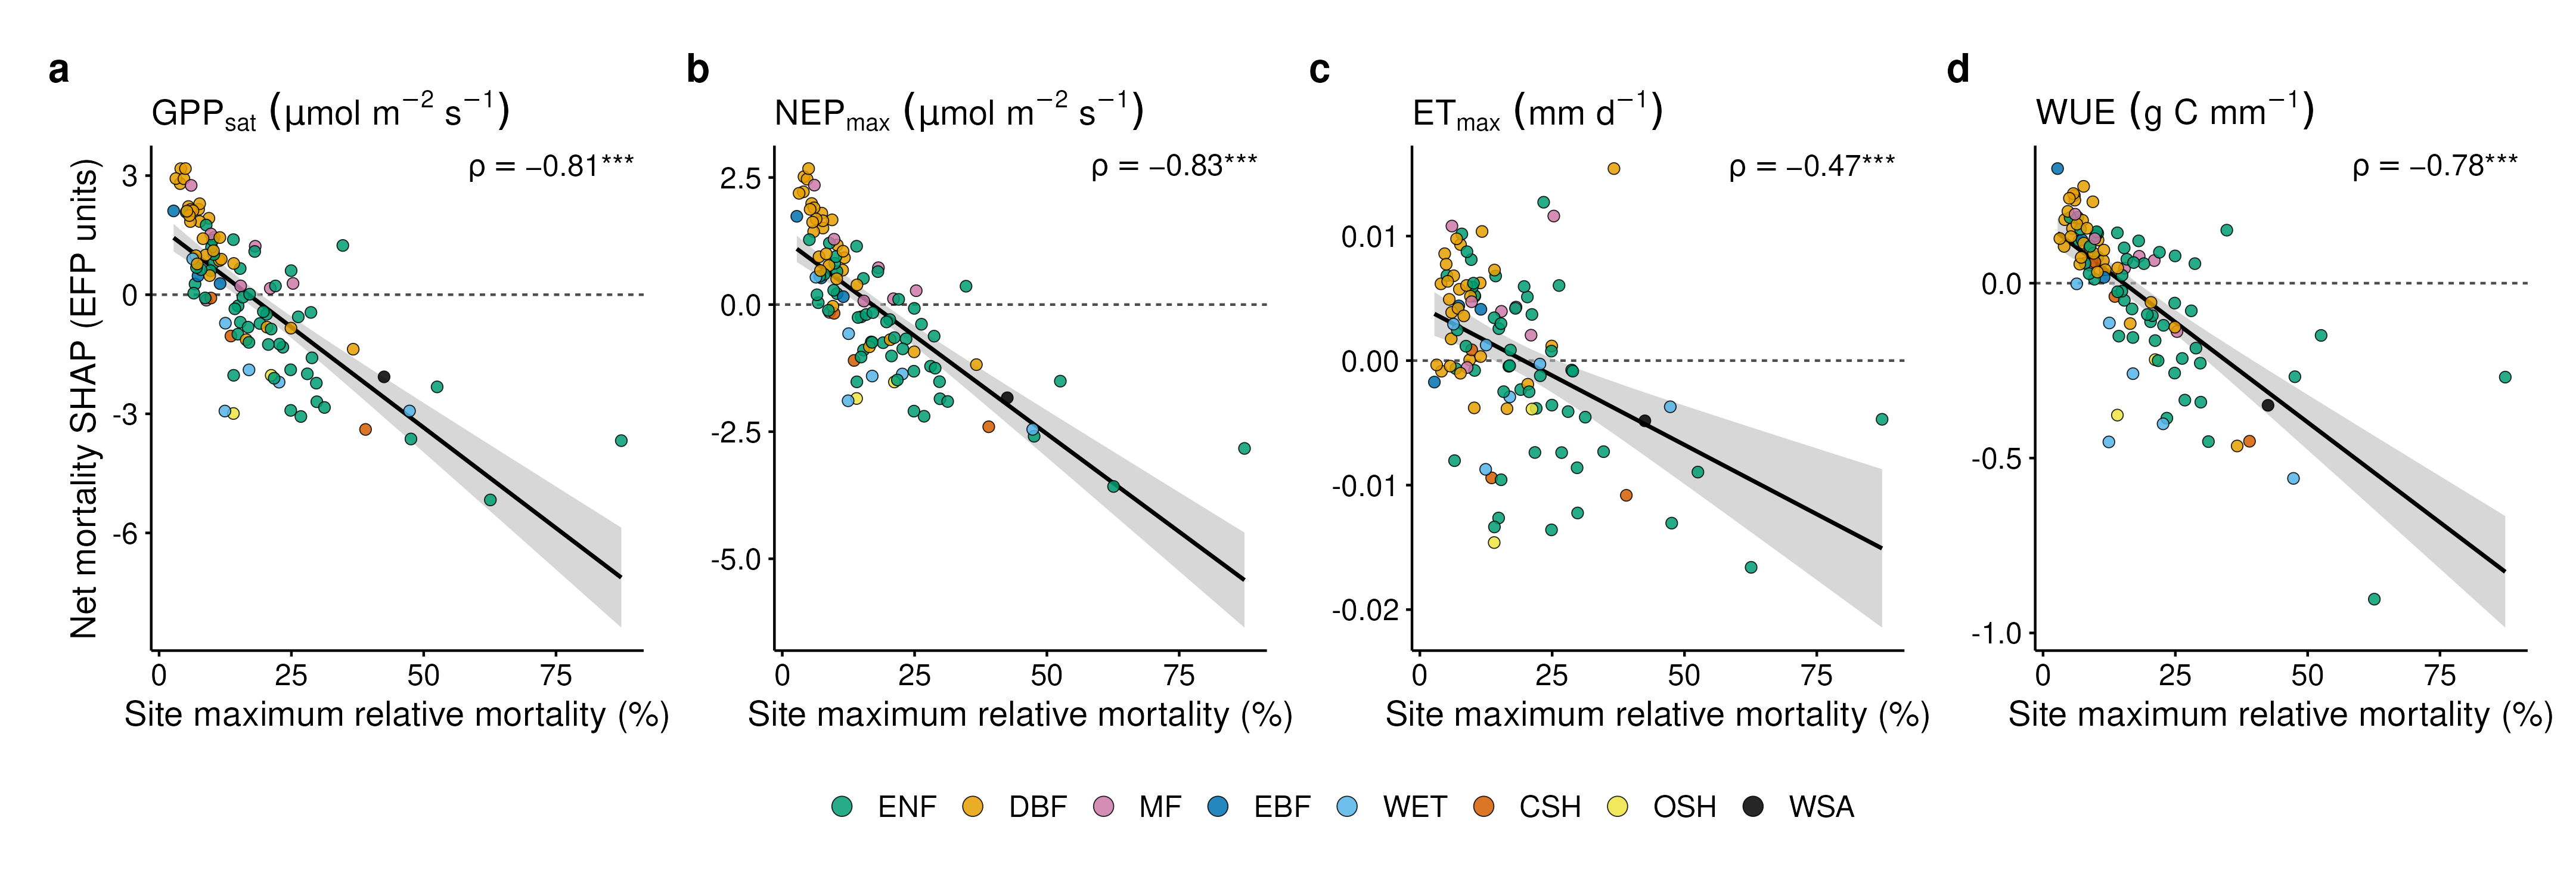
\includegraphics[width=\linewidth]{figures/fig5_relmort_direction_24m_AG.png}\\[2pt]
\parbox{\linewidth}{{\small \textbf{Fig.\ 5} $|$ \textbf{The direction of the mortality effect follows the amount of mortality.} Net mortality SHAP per site (as in Fig.~3) against the site's maximum relative mortality for GPP$_\mathrm{sat}$ (\textbf{a}), NEP$_\mathrm{max}$ (\textbf{b}), ET$_\mathrm{max}$ (\textbf{c}) and WUE (\textbf{d}); AutoGluon, C+T+M, 24-month window; $n$ = 101 sites coloured by IGBP class (abbreviations as in Fig.~1). Black line, linear fit with 95\,\% confidence band; dashed line, zero; $\rho$, Spearman rank correlation, Benjamini--Hochberg corrected across the four panels ($^{*}$\,$q<0.05$, $^{**}$\,$q<0.01$, $^{***}$\,$q<0.001$).}}
\end{center}


\textbf{Circularity check.} Refitting each property without the climate variables in its own formula (radiation for GPP$_{sat}$, air temperature for ET$_{max}$ and WUE) leaves the skill and the main mortality results essentially unchanged (Appendix~A8).

\textbf{Mortality metrics}
\begin{itemize}
  \item The mortality block contains five metrics (absolute deadwood, relative deadwood, deadwood gain, relative
        tree-cover loss, relative mortality) at five buffers. They are strongly correlated and largely interchangeable:
        removing any single metric changes the error by at most about 1\,\% (drop-column test, Appendix).
  \item \textbf{Relative mortality carries most of the effect} (added alone to C+T it gives 6.7--7.1\,\% of the 7.6--8.9\,\%
        NEP$_{max}$ error reduction of the full block) and has the largest SHAP share (26\,\%), so the figures use relative
        mortality only. The other metrics are in the Appendix.
\end{itemize}

